\documentclass[12pt,a4paper]{article}

\usepackage{caption}
\usepackage{geometry}
\usepackage{graphicx}
\usepackage{ragged2e}
\usepackage{multicol}
\usepackage{adjustbox}

\usepackage{courier}
\usepackage{graphicx}
\usepackage{caption}
\usepackage{mathptmx}
\usepackage{ragged2e}
\usepackage{xcolor}
\usepackage{listings}
\usepackage{enumitem}

\usepackage{listings}
\usepackage{xcolor}

\lstset{
  basicstyle=\ttfamily\normalfont\scriptsize,
  breakatwhitespace=true,         
  escapeinside={\%*}{*)},
  breakautoindent=true,
  breaklines=true,                 
  captionpos=b,                    
  keepspaces=false,                 
  showspaces=false,                
  showstringspaces=false,
  showtabs=false,                  
  frame=single,
  numbers=none,
  stepnumber=1,% the step between two line-numbers. If it's 1 each line will be numbered
  tabsize=2
}

% Bash
\lstdefinelanguage{Bash}{
  morekeywords={
    if,then,else,elif,fi,for,while,do,done,case,esac,export
  },
  sensitive=true,
  morecomment=[l]\#,
  morestring=[b]",
}

% C
\lstdefinelanguage{C}{
  morekeywords={
    auto,break,case,char,const,continue,default,do,double,else,
    enum,extern,for,if,int,long,register,return,switch,typedef,
    unsigned,void,volatile,while
  },
  sensitive=true,
  morecomment=[l]//,
  morecomment=[s]/* */ ,
  morestring=[b]",
}

% C++
\lstdefinelanguage{C++}{
  morekeywords={
    alignas,alignof,and,asm,auto,bitand,bitor,bool,break,case,
    class,compl,const,constexpr,continue,decltype,default,delete,
    do,double,else,enum,explicit,false,for,friend,goto,if,inline,
    int,long,mutable namespace,new noexcept,operator,private,
    protected,public,register,return,short,signed,sizeof,
    static,static_assert,static_cast,struct,switch,template,this,
    thread_local,throw,true,try,typedef,typeid,typename,union,
    unsigned,using,virtual,void,volatile,wchar_t,while
  },
  sensitive=true,
  morecomment=[l]//,
  morecomment=[s]/* */ ,
  morestring=[b]",
}

% Java
\lstdefinelanguage{Java}{
  morekeywords={
    abstract,assert,boolean,break,byte,case,catch,char,class,
    const,continue,default,do,double,else,enum,extends,final,
    finally,float, for,goto,if,implements,import,instanceof,int,
    interface,long,native,new, null,package,private,protected,
    public,return,short,static,strictfp, super,switch,
    synchronized,this,throw,throws,transient,true,try,void,
    volatile,while
  },
  sensitive=true,
  morestring=[b]",
}

% Go
\lstdefinelanguage{Go}{
  morekeywords={
    break,case,chan,const,continue,
    default,defer,else,fallthrough,
    for,function,goto,if,import,interface,
    map,package,range,return,select,struct,
    switch,type,var},
  sensitive=true,
  morecomment=[l]//,
  morecomment=[s]/* */ ,
  morestring=[b]",
}

% PHP
\lstdefinelanguage{PHP}{
  morekeywords={
    __halt_compiler,abstract,alias,arguments,break,case,class,
    clone,const,continue,declare,default,die,do,echo,else,elseif,
    empty,endswitch,eval,exit,extends,final,finally,for,foreach,
    function,global,goto,if,implements,include,include_once,
    instanceof,insteadof,interface,is,isset,list,namespace,
    print,private,protected,public,return,static,switch,throw,
    trait,try,unset,use,var,while,yield
  },
  sensitive=true,
  morecomment=[l]//,
  morecomment=[s]/* */ ,
  morestring=[b]",
}

% Javascript
\lstdefinelanguage{JavaScript}{
    morekeywords={abstract,arguments,await,boolean,break,byte,
    case,catch,class,const,continue,debugger,default,delete,do,
    double,else,enum,eval,export,extends,false,finally,for,function,
    global,if,implements,import,in,instanceof,int,let,match,namespace,
    NaN,private,protected,public,return,super,switch,throw,throws,true,
    try,typeof,var,void,yield
  },
  sensitive=true,
  morecomment=[l]//,
  morecomment=[s]/* */ ,
  morestring=[b]",
}



\geometry{margin=2cm}
\graphicspath { {./img/} }

\pagenumbering{gobble}
\date{}

\captionsetup[figure]{labelformat=empty}
\renewcommand\contentsname {\Large{\textbf{DAFTAR ISI}} }
\renewcommand{\refname}{}

\title{

  \large{\textbf{LAPORAN}}

  \large{\textbf{Penelusuruan Rute Terpendek Antara Kota di Australia Menggunakan Algoritma A*}}

  {\large{Diajukan untuk Memenuhi Tugas Mata Kuliah Kecerdasan Buatan}}

  {\vspace{1cm}}

  \normalsize{Radinal Shidiq Saragih}

  {\vspace{0.5cm}}

  \normalsize{IF C 2023}

  {\vspace{0.5cm}}

  \normalsize{5520123104}

  {\vspace{1cm}}

  {
\includegraphics[scale=1.8]{LogoFakultas.jpeg}}

  {\vspace{2cm}}

  {\large{PROGRAM STUDI TEKNIK INFORMATIKA}}

  {\large{FAKULTAS TEKNIK}}

  {\large{UNIVERSITAS SURYAKANCANA}}

  {\large{CIANJUR}}

  {\small{2025}}
}

\begin{document}

\begin{titlepage}
  \maketitle
\end{titlepage}

\pagenumbering{roman}

\begin{center}
  \section*{KATA PENGANTAR}
\end{center}
\setcounter{section}{1}
\setcounter{subsection}{0}
\addcontentsline{toc}{section}{KATA PENGANTAR}{}

\vspace{1cm}

Puji dan syukur saya panjatkan ke hadirat Tuhan Yang Maha Esa atas rahmat
dan karunia-Nya sehingga laporan ini dapat diselesaikan dengan baik.
Laporan ini membahas konsep algoritma A* serta penerapannya
dalam studi kasus pencarian jalur optimal. Penulisan laporan ini
bertujuan untuk memberikan pemahaman tentang bagaimana algoritma ini bekerja
serta faktor-faktor yang memengaruhi efisiensinya.

Kami menyadari bahwa dalam penyusunan laporan ini masih terdapat kekurangan.
Oleh karena itu, saya terbuka terhadap kritik dan saran yang membangun guna
meningkatkan kualitas laporan ini di masa mendatang.

Akhir kata, saya mengucapkan terima kasih kepada semua pihak yang telah membantu
dalam penyusunan makalah ini, terutama kepada dosen
pengampu mata kuliah serta rekanrekan yang telah
memberikan dukungan dan masukan berharga.

\vspace{1cm}

\begin{flushright}
  Cianjur, Maret 2025

  \vspace{0.5cm}

  Penulis
\end{flushright}

\newpage

\begin{center}
  \tableofcontents
\end{center}
\addcontentsline{toc}{section}{DAFTAR ISI}{}
\vspace{1cm}

\newpage

\pagenumbering{arabic}

\begin{center}
  \large{\textbf{BAB I}}

  \section*{PENDAHULUAN}
\end{center}
\addcontentsline{toc}{section}{BAB I PENDAHULUAN}{}
\vspace{1cm}

\subsection{Latar Belakang}
Algoritma A* (A-star) adalah salah satu metode pencarian yang banyak
digunakan karena kemampuannya menemukan jalur terpendek secara efisien
dengan mengombinasikan eksplorasi dan estimasi biaya ke tujuan.

Laporan ini membahas konsep dasar dari algoritma A*, termasuk bagaimana
heuristik memengaruhi kinerja pencarian, serta studi kasus penerapannya
dalam suatu skenario tertentu. Studi kasus ini bertujuan untuk mengamati
bagaimana A* menelusuri jalur dari titik awal ke titik tujuan.
Dengan demikian, diharapkan laporan ini dapat memberikan wawasan
lebih dalam mengenai bagaimana A* dapat digunakan secara optimal
dalam berbagai permasalahan pencarian jalur.


\subsection{Rumusan Masalah}

\begin{enumerate}
  \item Bagaimana contoh penerapan Algoritma A*?
  \item Bagaimana dampak dari estimasi heuristik terhadap penelusuran?
  \item Bagaimana menghasilkan nilai estimasi yang tepat?
\end{enumerate}


\subsection{Tujuan}

\begin{enumerate}
\item Mempraktekan penelusuran A*
\item Memahami cara kerja algoritma A*
\item Memahami karakteristik algoritma A*
\item Memahami cara menghasilkan esitimasi heuristik
\item Mengetahui potensi yang dimiliki algoritma A*
\end{enumerate}


\newpage

\begin{center}
  \large{\textbf{BAB II}}

  \section*{PEMBAHASAN}
\end{center}
\addcontentsline{toc}{section}{BAB II PEMBAHASAN}{}
\vspace{1cm}

\subsection{Konsep Algoritma Pencarian A*}

A* (A-star) adalah algoritma pencarian yang digunakan untuk menemukan jalur
terpendek dalam graf atau ruang pencarian. Algoritma ini menggabungkan
keunggulan dari Breadth-First Search (BFS) dan Dijkstra’s Algorithm
dengan menggunakan fungsi evaluasi f(n) = g(n) + h(n), di mana g(n)
adalah biaya dari titik awal ke node saat ini, dan h(n) adalah estimasi
biaya dari node saat ini ke tujuan (heuristik). A* bekerja dengan menelusuri
jalur yang memiliki nilai f(n) terendah terlebih dahulu, sehingga lebih optimal
dalam menemukan solusi dibandingkan dengan pencarian buta.

Nilai Heuristik dalam A* untuk mendapatkan estimasi yang membantu
mempercepat dan menambahkan akurasi pencarian.
Terdapat beragam fungsi heuristik yang dapat digunakan, antaralain Euclidean
Distance, Manhattan Distance, Equirectangular Approximation dan masih
banyak lagi.

Peran esitmasi heuristik dalam pencarian dengan algoritma A* berpengaruh
besar karena dapat memberikan hasil akhir yang lebih optimal dibanding
tidak menggunakannya.

\subsection{Studi Kasus} 

\begin{center}
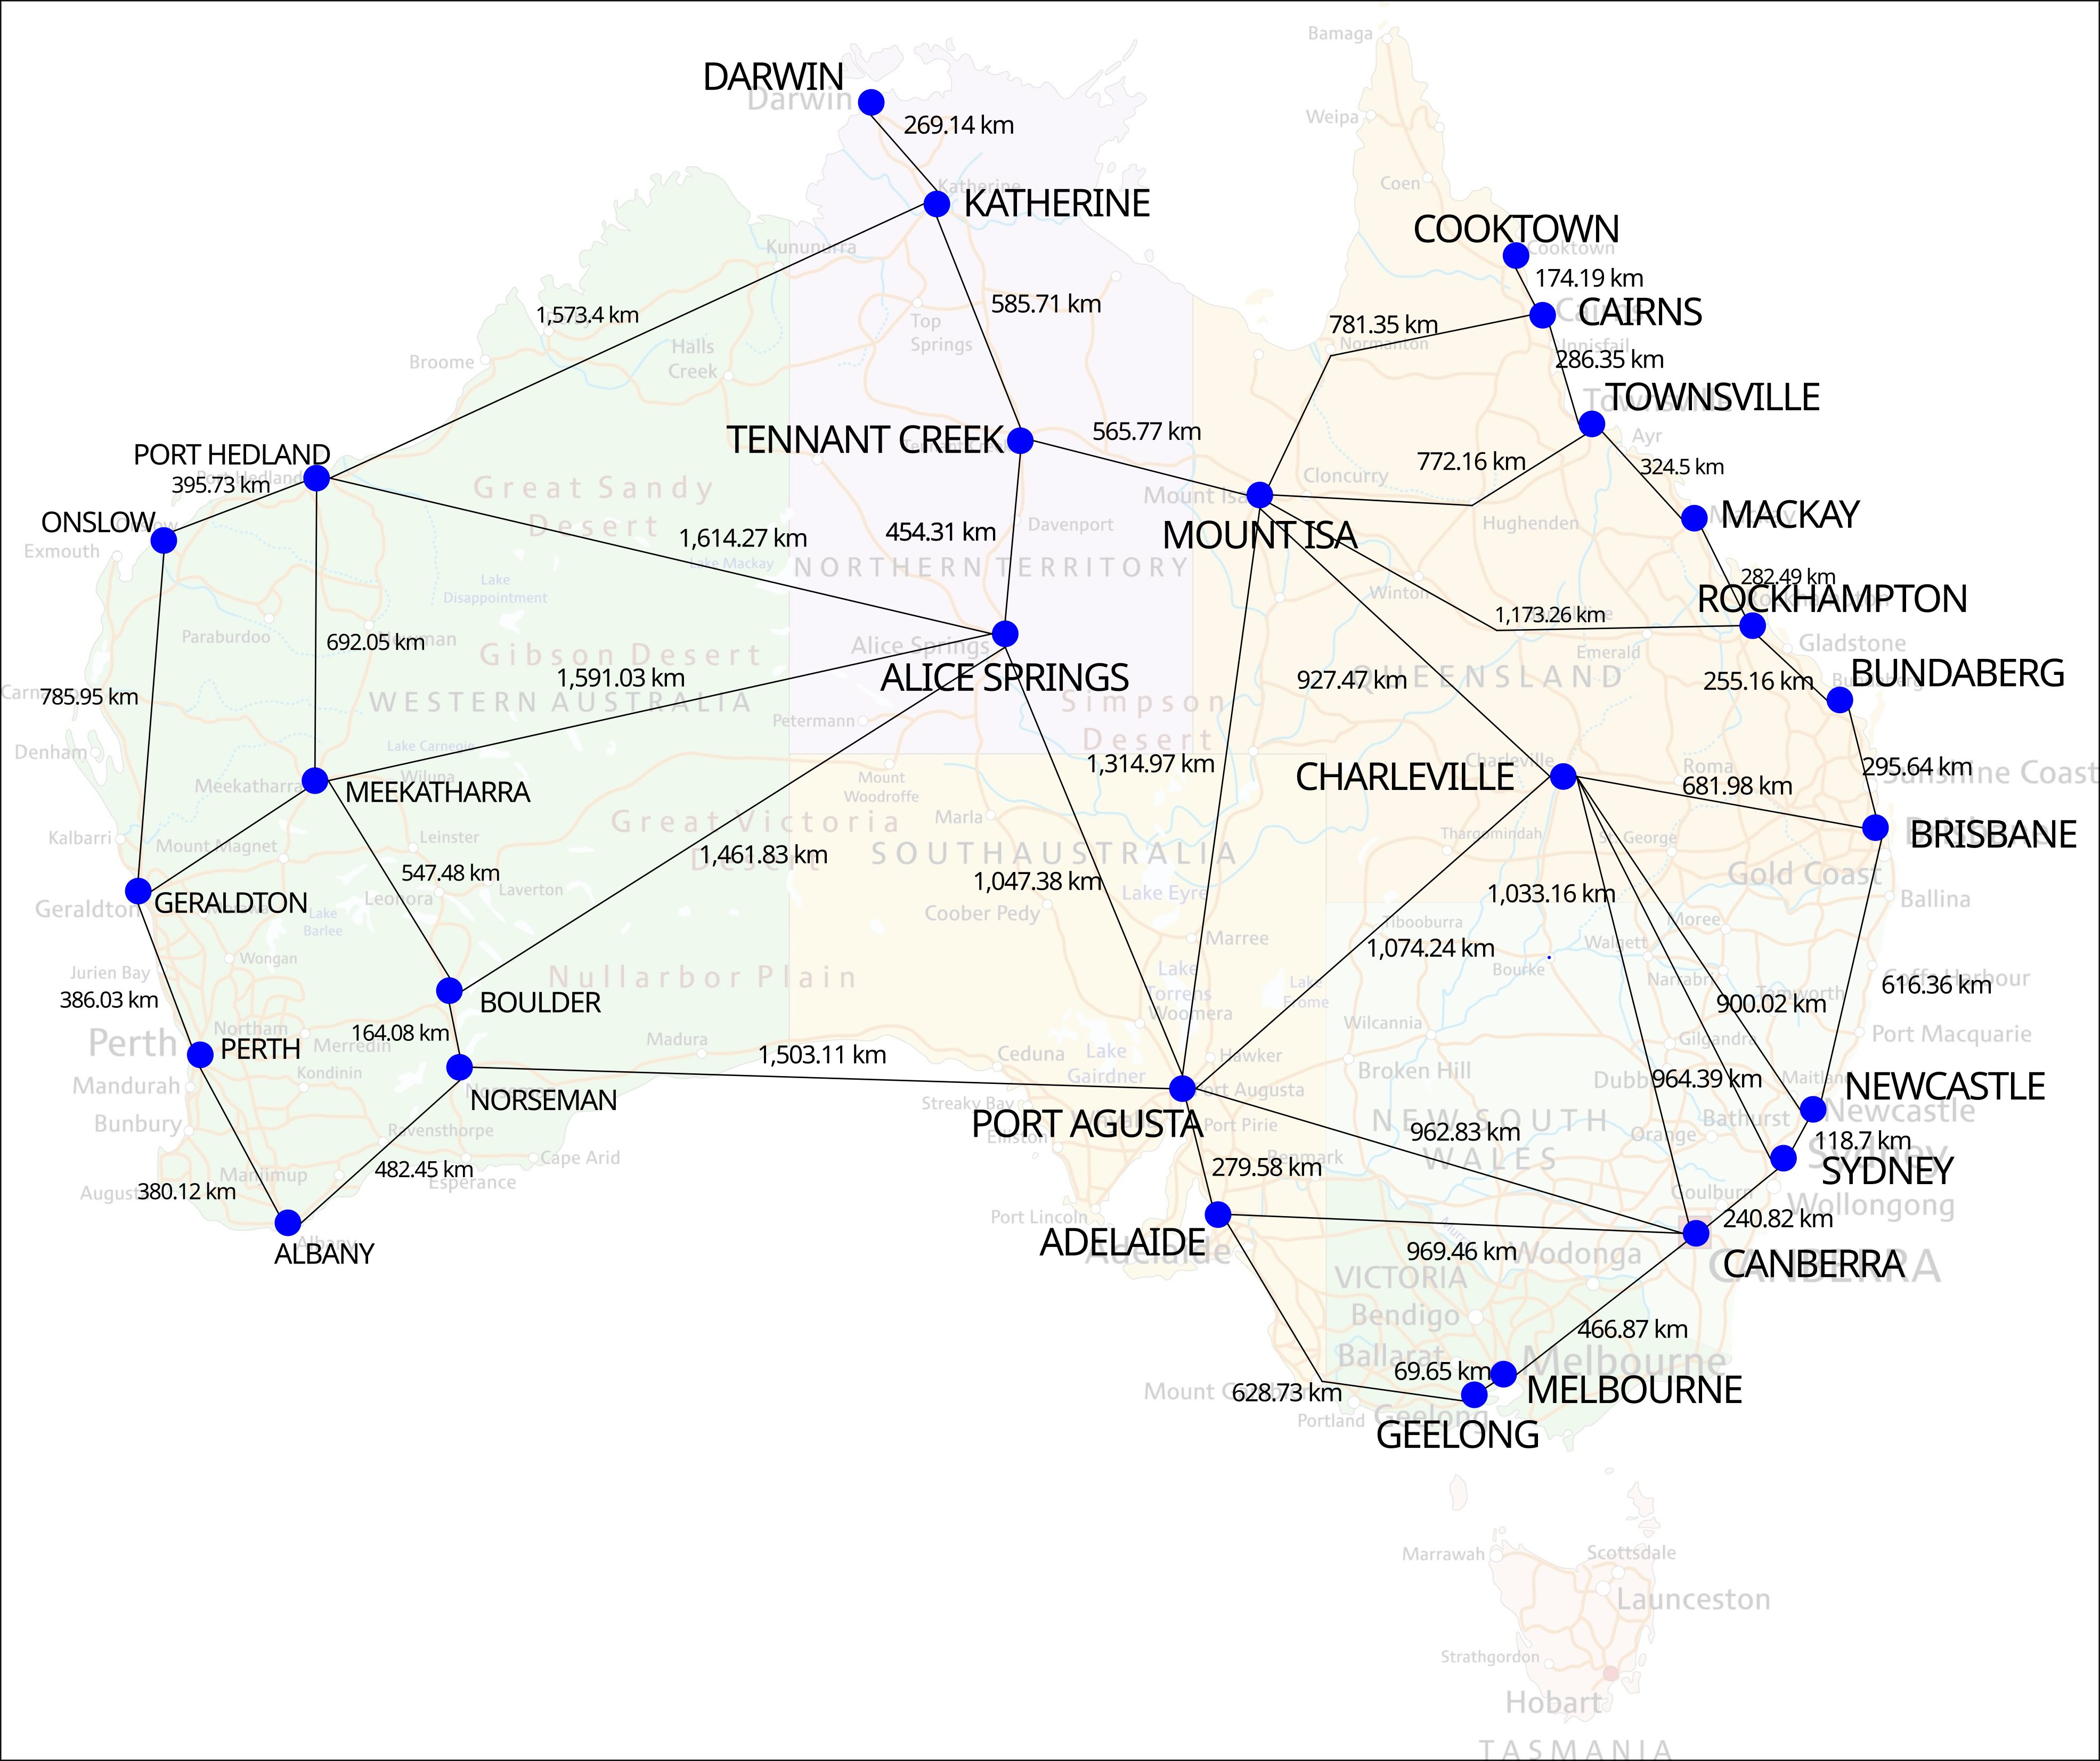
\includegraphics[scale=0.1]{australia.png}
\end{center}

Di dalam studi kasus yang saya pilih, terdapat masalah yaitu
untuk mencari jalur terpendek dari Darwin menuju Canberra. Studi kasus
ini melibatkan 27 kota.

\subsubsection{Perhitungan Nilai Heuristik}

Nilai heuristik akan didapatkan dari fungsi \emph{Equirectangular Approximation},
dengan rumus sebagai berikut.

\subsubsection*{Rumus}

\begin{center}
\[ 
  X = \Delta lng \cdot \cos \left( \frac{lat_1 + lat_2}{2} \right) 

  Y = \Delta lat 

  d = R \cdot \sqrt{X^2 + Y^2} 

\]
\end{center}

\subsubsection*{Keterangan}

\begin{itemize}
    \item \(\Delta lng = lng_2 - lng_1\)
    \item \(\Delta lat = lat_2 - lat_1\)
    \item \(X\) = Perbedaan posisi dalam koordinat longitude
    \item \(Y\) = Perbedaan posisi dalam koordinat latitude
    \item \(Lat\) = Latitude dalam radian:
    \[
    \text{Latitude} \times 0.0174532925
    \]
    \item \(Lng\) = Longitude dalam radian:
    \[
    \text{Longitude} \times 0.0174532925
    \]
    \item \(d\) = Jarak antara dua titik dalam kilometer
    \item \(R\) = Jari-jari bumi (\(6.371\) km)
\end{itemize}

Berikut adalah posisi latitude dan longitude dari kota-kota di studi kasus ini.

\begin{table}[h]
    \centering
    \begin{tabular}{|c|c|c|c|}
        \hline
        \textbf{Nama Kota} & \textbf{Latitude} & \textbf{Longitude} \\
        \hline
        Adelaide & 34.9285 & 138.6007 \\
        Albany & 35.0269 & 117.8831 \\
        Alice Springs & 23.698 & 133.8807 \\
        Boulder & 30.7826 & 121.4889  \\
        Brisbane & 27.4698 & 153.0251  \\
        Bundaberg & 24.8662 & 152.3489  \\
        Cairns & 16.9203 & 145.771  \\
        Canberra & 35.2809 & 149.13  \\
        Charleville & 26.4075 & 146.2413  \\
        Cooktown & 15.467 & 145.2519  \\
        Darwin & 12.4634 & 130.8456  \\
        Geelong & 38.1499 & 144.3617  \\
        Geraldton & 28.7744 & 114.608  \\
        Katherine & 14.465 & 132.2635  \\
        Mackay & 21.1411 & 149.186  \\
        Meekatharra & 26.5916 & 118.4933  \\
        Melbourne & 37.8136 & 144.9631  \\
        Mount Isa & 20.725 & 139.4973  \\
        Newcastle & 32.9283 & 151.7817  \\
        Norseman & 32.1968 & 121.7792  \\
        Onslow & 21.6389 & 115.1128  \\
        Perth & 31.9505 & 115.8605  \\
        Port Augusta & 32.4911 & 137.765  \\
        Port Hedland & 20.3104 & 118.606  \\
        Rockhampton & 23.379 & 150.511  \\
        Sydney & 33.8688 & 151.2093  \\
        Tennant Creek & 19.6489 & 134.1917  \\
        Townsville & 19.2589 & 146.8169  \\
        \hline
    \end{tabular}
\end{table}

Untuk mendapatkan nilai heuristik dari suatu kota dapat 
dilakukan sebagai berikut.

Misalkan untuk mencari nilai heuristik dari Kota Cooktown,
yang terdapat pada koordinasi sebagai berikut.

\[Latitude: 15.4670 \]

\[Longitude: 145.2519\]

Karena goal state atau tujuan akhir dari pencarian adalah Kota Canberra, maka
kita akan juga membutuhkan koordinasi dari goal state, yaitu.

\[ Latitude: 35.2809  \]

\[ Longitude:149.1300 \]

Setelah kedua kota didapatkan kita sudah dapat melakukan perhitungan, yaitu
seperti berikut.

\subsubsection*{Diketauhi}

\[lat_1: 15.4670\]
\[lng_1: 145.2519\]
\[lat_2: 35.2809\]
\[lng_2: 149.1300\]


\subsubsection*{Rubah Kooordinat menjadi radian}

\[lat_1: 15.4670 * 0.0174532925 = 0.27\]
\[lng_1: 145.2519 * 0.0174532925 = 2.5351\]
\[lat_2: 35.2809 * 0.0174532925 = 0.6158\]
\[lng_2: 149.1300 * 0.0174532925 = 2.6028\]

\subsubsection*{Hitung Nilai Heuristik}

\[\Delta lng = 2.6028 - 2.5351 = 0.0677\]
\[\Delta lat = 0.6158 - 0.27 = 0.3458\]

\[X = 2.6028 \cdot \cos \left( \frac{0.2677 + 0.6158}{2} \right) = 0.0612\]

\[Y = 0.3458\]

\[d = 6371 \cdot \sqrt{0.0612^2 + 0.3458^2} = 2237.3287 km\]

Maka nilai heuristik dari kota Cooktown dengan Canberra adalah 15143.78km.

Setelah melakukan operasi yang serupa untuk tiap koordinat kota maka didapatkan sebagai berikut.

\begin{table}[h]
    \centering
    \begin{tabular}{|c|c|c|c|}
        \hline
        \textbf{Nama Kota} & \textbf{Latitude} & \textbf{Longitude} & \textbf{Jarak} \\
        \hline
        Adelaide & 34.9285 & 138.6007 & 959.0122km \\
        Albany & 35.0269 & 117.8831 & 2840.9736km \\
        Alice Springs & 23.698 & 133.8807 & 1958.7422km \\
        Boulder & 30.7826 & 121.4889 & 2624.5242km \\
        Brisbane & 27.4698 & 153.0251 & 944.5546km \\
        Bundaberg & 24.8662 & 152.3489 & 1198.92km \\
        Cairns & 16.9203 & 145.771 & 2069.222km \\
        Canberra & 35.2809 & 149.13 & 0.0km \\
        Charleville & 26.4075 & 146.2413 & 1024.6996km \\
        Cooktown & 15.467 & 145.2519 & 2237.3287km \\
        Darwin & 12.4634 & 130.8456 & 3145.6881km \\
        Geelong & 38.1499 & 144.3617 & 531.0866km \\
        Geraldton & 28.7744 & 114.608 & 3333.8147km \\
        Katherine & 14.465 & 132.2635 & 2872.8145km \\
        Mackay & 21.1411 & 149.186 & 1572.3733km \\
        Meekatharra & 26.5916 & 118.4933 & 3077.4426km \\
        Melbourne & 37.8136 & 144.9631 & 466.6165km \\
        Mount Isa & 20.725 & 139.4973 & 1874.735km \\
        Newcastle & 32.9283 & 151.7817 & 357.9175km \\
        Norseman & 32.1968 & 121.7792 & 2552.4918km \\
        Onslow & 21.6389 & 115.1128 & 3654.7069km \\
        Perth & 31.9505 & 115.8605 & 3103.2473km \\
        Port Augusta & 32.4911 & 137.765 & 1093.6031km \\
        Port Hedland & 20.3104 & 118.606 & 3432.7048km \\
        Rockhampton & 23.379 & 150.511 & 1330.637km \\
        Sydney & 33.8688 & 151.2093 & 247.0848km \\
        Tennant Creek & 19.6489 & 134.1917 & 2279.1276km \\
        Townsville & 19.2589 & 146.8169 & 1796.587km \\
        \hline
    \end{tabular}
\end{table}

Setelah diketauhi nilai-nilai heuristik penelusuran sudah dapat dilakukan.

\newpage

\subsection{Penelusuran Algoritma A*}

Sifat dari Algoritma A* adalah Greedy Best-First Search, maka semua node
akan dikunjungi dengan node dengan biaya terkecil didahulukan. Biaya didapatkan
dari real-cost ditambah dengan nilai heuristik.

\[
  f(n) = g(n) + h(n)
\]

\begin{itemize}
  \item g(n)

    Biaya aktual dari titik awal ke titik saat ini (node n).

  \item h(n)

    Biaya perkiraan (heuristik) dari titik saat ini (n) ke titik tujuan.

  \item n(n)

    Total biaya perkiraan, nilai ini digunakan untuk menentukan urutan ekspansi node.
\end{itemize}

\subsubsection*{Alur Penelusuran}

\subsubsection*{Langkah 1}

\begin{itemize}
    \item \textbf{OPEN}: KATHERINE
    \item \textbf{CLOSED}: DARWIN
\end{itemize}

DARWIN ke KATHERINE:  
\[
f(n) = 269.14 + 2871.8145 = 3140.9545
\]

DARWIN statusnya \textbf{CLOSED} karena merupakan node awal penelusuran.  
Karena hanya ada KATHERINE yang terhubung dengan DARWIN, maka KATHERINE dinyatakan \textbf{OPEN}.  

\subsubsection*{Langkah 2}

\begin{itemize}
    \item \textbf{OPEN}: TENNANT CREEK, PORT HEDLAND
    \item \textbf{CLOSED}: KATHERINE, DARWIN
\end{itemize}

KATHERINE memiliki dua tetangga, yaitu PORT HEDLAND dan TENNANT CREEK, dengan biaya sebagai berikut:

\[
f(\text{KATHERINE} \to \text{PORT HEDLAND}) = 1573.4 + 118.606 = 1692.006
\]

\[
f(\text{KATHERINE} \to \text{TENNANT CREEK}) = 585.71 + 2279.1276 = 2864.8376
\]

Karena biaya terkecil adalah PORT HEDLAND, maka akan ditelusuri terlebih dahulu pada tahap berikutnya.  

\subsubsection*{Langkah 3}

\begin{itemize}
    \item \textbf{OPEN}: MEEKATHARRA, ONSLOW, ALICE SPRINGS, TENNANT CREEK
    \item \textbf{CLOSED}: PORT HEDLAND, KATHERINE, DARWIN
\end{itemize}

PORT HEDLAND memiliki empat tetangga, tetapi karena KATHERINE telah ditelusuri, maka diabaikan.  
Biaya menuju tetangga lainnya adalah:

\[
f(\text{PORT HEDLAND} \to \text{ONSLOW}) = 395.73 + 3654.7069 = 4050.4369
\]

\[
f(\text{PORT HEDLAND} \to \text{MEEKATHARRA}) = 692.05 + 3077.4426 = 3769.4925
\]

\[
f(\text{PORT HEDLAND} \to \text{ALICE SPRINGS}) = 1614.27 + 1958.7422 = 3573.0122
\]

Karena biaya terkecil adalah ALICE SPRINGS, maka akan ditelusuri terlebih dahulu.  

\subsubsection*{Langkah 4}

\begin{itemize}
    \item \textbf{OPEN}: PORT AUGUSTA, BOULDER, MEEKATHARRA, ONSLOW, ALICE SPRINGS, TENNANT CREEK
    \item \textbf{CLOSED}: ALICE SPRINGS, PORT HEDLAND, KATHERINE, DARWIN
\end{itemize}

ALICE SPRINGS memiliki beberapa tetangga dengan biaya sebagai berikut:

\[
f(\text{ALICE SPRINGS} \to \text{TENNANT CREEK}) = 465.31 + 2279.127 = 2744.437
\]

\[
f(\text{ALICE SPRINGS} \to \text{MEEKATHARRA}) = 1591.03 + 3077.4426 = 4469.4726
\]

\[
f(\text{ALICE SPRINGS} \to \text{BOULDER}) = 1461.83 + 2624.5242 = 4086.3541
\]

\[
f(\text{ALICE SPRINGS} \to \text{PORT AUGUSTA}) = 1314.97 + 1093.6031 = 2408.5731
\]

Karena biaya terkecil adalah PORT AUGUSTA, maka akan ditelusuri terlebih dahulu.  

\subsubsection*{Langkah 5}

\begin{itemize}
    \item \textbf{OPEN}: CANBERRA, ADELAIDE, CHARLEVILLE, MOUNT ISA, NORSEMAN, BOULDER, MEEKATHARRA, ONSLOW, ALICE SPRINGS, TENNANT CREEK
    \item \textbf{CLOSED}: PORT AUGUSTA, ALICE SPRINGS, PORT HEDLAND, KATHERINE, DARWIN
\end{itemize}

PORT AUGUSTA memiliki beberapa tetangga dengan biaya sebagai berikut:

\[
f(\text{PORT AUGUSTA} \to \text{ADELAIDE}) = 279.58 + 959.0122 = 1238.5922
\]

\[
f(\text{PORT AUGUSTA} \to \text{CANBERRA}) = 962.83 + 0 = 962.83
\]

Karena \textbf{Goal State} (CANBERRA) telah tercapai, maka penelusuran dihentikan.  

\subsection{Hasil Penelusuran Algoritma A*}

Maka bedasarkan hasil penelusuran, jalur terpendek dari DARWIN menuju CANBERRA adalah.
DARWIN,  PORT HELAND, ALICE SPRINGS, PORT AGUSTA, CANBERRA.

\newpage

\begin{center}
  \large{\textbf{BAB 4}}

  \section*{KESIMPULAN}
\end{center}
\addcontentsline{toc}{section}{BAB V KESIMPULAN}{}
\vspace{1cm}

Kesimpulannya penelusuran dengan A* merupakan salah satu metode yang sederhana
untuk menghasilkan jalur yang teroptimal dari dua buah titik, dan penerapan
algoritma ini sangat beragam tidak hanya untuk untuk mengkalkulasi jalur dipeta.

\end{document}
